\documentclass[english]{tktltiki2}

% --- General packages ---

\usepackage[utf8]{inputenc}
\usepackage[T1]{fontenc}
\usepackage{lmodern}
\usepackage{microtype}
%\usepackage[table,xcdraw]{xcolor}    % loads also »colortbl«
\usepackage{listings}
\usepackage{tabularx}
%\usepackage{minted}
%\usepackage{tcolorbox}
%\usepackage{etoolbox}
%\BeforeBeginEnvironment{minted}{\begin{tcolorbox}}%
%\AfterEndEnvironment{minted}{\end{tcolorbox}}%

\usepackage{amsfonts,amsmath,amssymb,amsthm,booktabs,enumitem,graphicx}
\usepackage{tocloft}
%\usepackage{relsize}
\usepackage[pdftex,hidelinks]{hyperref}
\usepackage[title]{appendix}
%\usepackage{tabularx}
%\usepackage[table]{xcolor}    % loads also »colortbl«
%\usepackage{float}

%\listfiles

\linespread{1.3}

\setlength{\intextsep}{18pt plus 2.0pt minus 2.0pt}

\lstset{%
  language=[LaTeX]TeX,
  basicstyle=\ttfamily,
  breaklines=true,
  columns=fullflexible,
}

%\setlength{\arrayrulewidth}{0.6pt}

% Automatically set the PDF metadata fields
\makeatletter
\AtBeginDocument{\hypersetup{pdftitle = {\@title}, pdfauthor = {\@author}}}
\makeatother

% --- Language-related settings ---
%
% these should be modified according to your language

% babelbib for non-english bibliography using bibtex
\usepackage[fixlanguage]{babelbib}
\selectbiblanguage{english}

% add bibliography to the table of contents
\usepackage[nottoc]{tocbibind}
% tocbibind renames the bibliography, use the following to change it back

\declarebtxcommands{english}{%
    \def\btxurldatecomment#1{ [#1]}%
}

% --- tktltiki2 options ---
%
% The following commands define the information used to generate title and
% abstract pages. The following entries should be always specified:

\title{Mining a Bird Observatory Dataset}
\author{Mikko Koho}
\date{\today}
\level{Technical report}

\abstract{
This report examines the use of data mining techniques to find interesting patterns from a bird observatory dataset.

The bird observations are modeled as an RDF Data Cube dataset and linked with weather data from nearby weather station in Hanko, Russarö and a bird taxon ontology. This RDF data is transformed to simpler formats for association analysis, by grouping together relevant pieces of information from the RDF datasets and related ontologies. This allows to analyse the information directly with pattern mining algorithms and association rule generation. Using these methods, we were able to find some interesting patterns from the dataset.

Data mining approach can be applied to nature observation datasets to find interesting patterns. Organising the data for pattern mining is however not trivial as there are numerous possible ways to do this.
}

\keywords{}
%\classification{
%\textbf{} \\
%\textit{} \\
%\\
%}
% classification according to ACM Computing Classification System (http://www.acm.org/about/class/)
                  % This is probably mostly relevant for computer scientists

% If the automatic page number counting is not working as desired in your case,
% uncomment the following to manually set the number of pages displayed in the abstract page:
%



\begin{document}
    
% --- Front matter ---

\frontmatter      % roman page numbering for front matter

\maketitle        % title page

\makeabstract     % abstract page

\tableofcontents  % table of contents

% --- Main matter ---

\mainmatter       % clear page, start arabic page numbering


%%%%%%%%%%%%%%%%%%%
\section{Introduction}
%%%%%%%%%%%%%%%%%%%

This report examines the use of data mining techniques~\cite{tan2006introduction} to find interesting patterns from a bird observatory dataset. Section 2 shows some related work. Section 3 explains the structure and content of the dataset. Section 4 explains the used analysis methods and section 5 lays out results obtained using those methods. Sections 6 and 7 provide conclusions and discussion.

First occurences of bird species names are written written with finnish, english and scientific names, to be more accessible to different audiences. The format used is <finnish name, \emph{scientific name}, english name>.


%%%%%%%%%%%%%%%%%%%
\section{Related work}
%%%%%%%%%%%%%%%%%%%

Kelling et al. have used exploratory analysis to find patterns in observational records of wintering birds in North America~\cite{kelling2009data}. They also lay out the importance of data-driven approaches in biodiversity research.
Caruana et al.~\cite{caruana2006mining} and Hochaka et al.~\cite{hochachka2007data} apply data mining and machine learning to bird observation datasets. Also other articles use classification models to predict occurence of bird species\cite{goetz2014relative, mentch2014ensemble}.

The dataset used in this report has already been presented in earlier work~\cite{koho-hyvonen-orni-2014, koho2015gradu}, including some exploratory analysis with visualizations.

%%%%%%%%%%%%%%%%%%%
\section{Dataset}
%%%%%%%%%%%%%%%%%%%

Hanko Bird Observatory, \emph{Halias}, is located at the southernmost tip of Finland in Hanko, Finland. Halias has been gathering bird observation data from 1979 onward and it has been used intensively in research~\cite{HangonJulkaisut}. However data mining or machine learning methods have been never applied to it, so these methods could perhaps uncover some interesting patterns in the data.

Gathering the data at Halias is highly standardized and main focus is on counting the daily migration of each bird species. Manning the station is based on volunteers, which causes some gaps in the data when no observers are present.
The dataset is not publicly available, but is available for research projects at request.

The data in original digital format consists of two Excel files, containing half a million rows of distinct daily counts per species for local and migrating birds from 1979 to 2009. Some rows contain a \emph{taxon} (plural \emph{taxa}) that is higher than species-level, for example a genus or a species pair.

However, in this case study we will be using a linked data publication made from the original dataset. The dataset has been transformed~\cite{koho-hyvonen-orni-2014, koho2015gradu} to RDF data model and linked with weather data from nearby weather station in Hanko, Russarö and a bird taxon ontology.
The linked dataset is structured using the RDF Data Cube Vocabulary~\cite{w3crdfdatacube}, containing distinct data cubes for both daily bird observations and daily weather observations. An example of the bird observation data in this format is given in figure \ref{fig: havaintograafi}.

The used bird taxon ontology~\cite{koho2015gradu} contains finnish conservation statuses for endangered species, a coarse measure of commonness at Halias and characteristics of many finnish species, such as size, beak color and plumage coloring. The taxon ontology is open and available\footnote{\url{http://www.ldf.fi/dataset/halias/rdf/halias_taxon_ontology.zip}}.

\begin{figure}[htb]
\centering
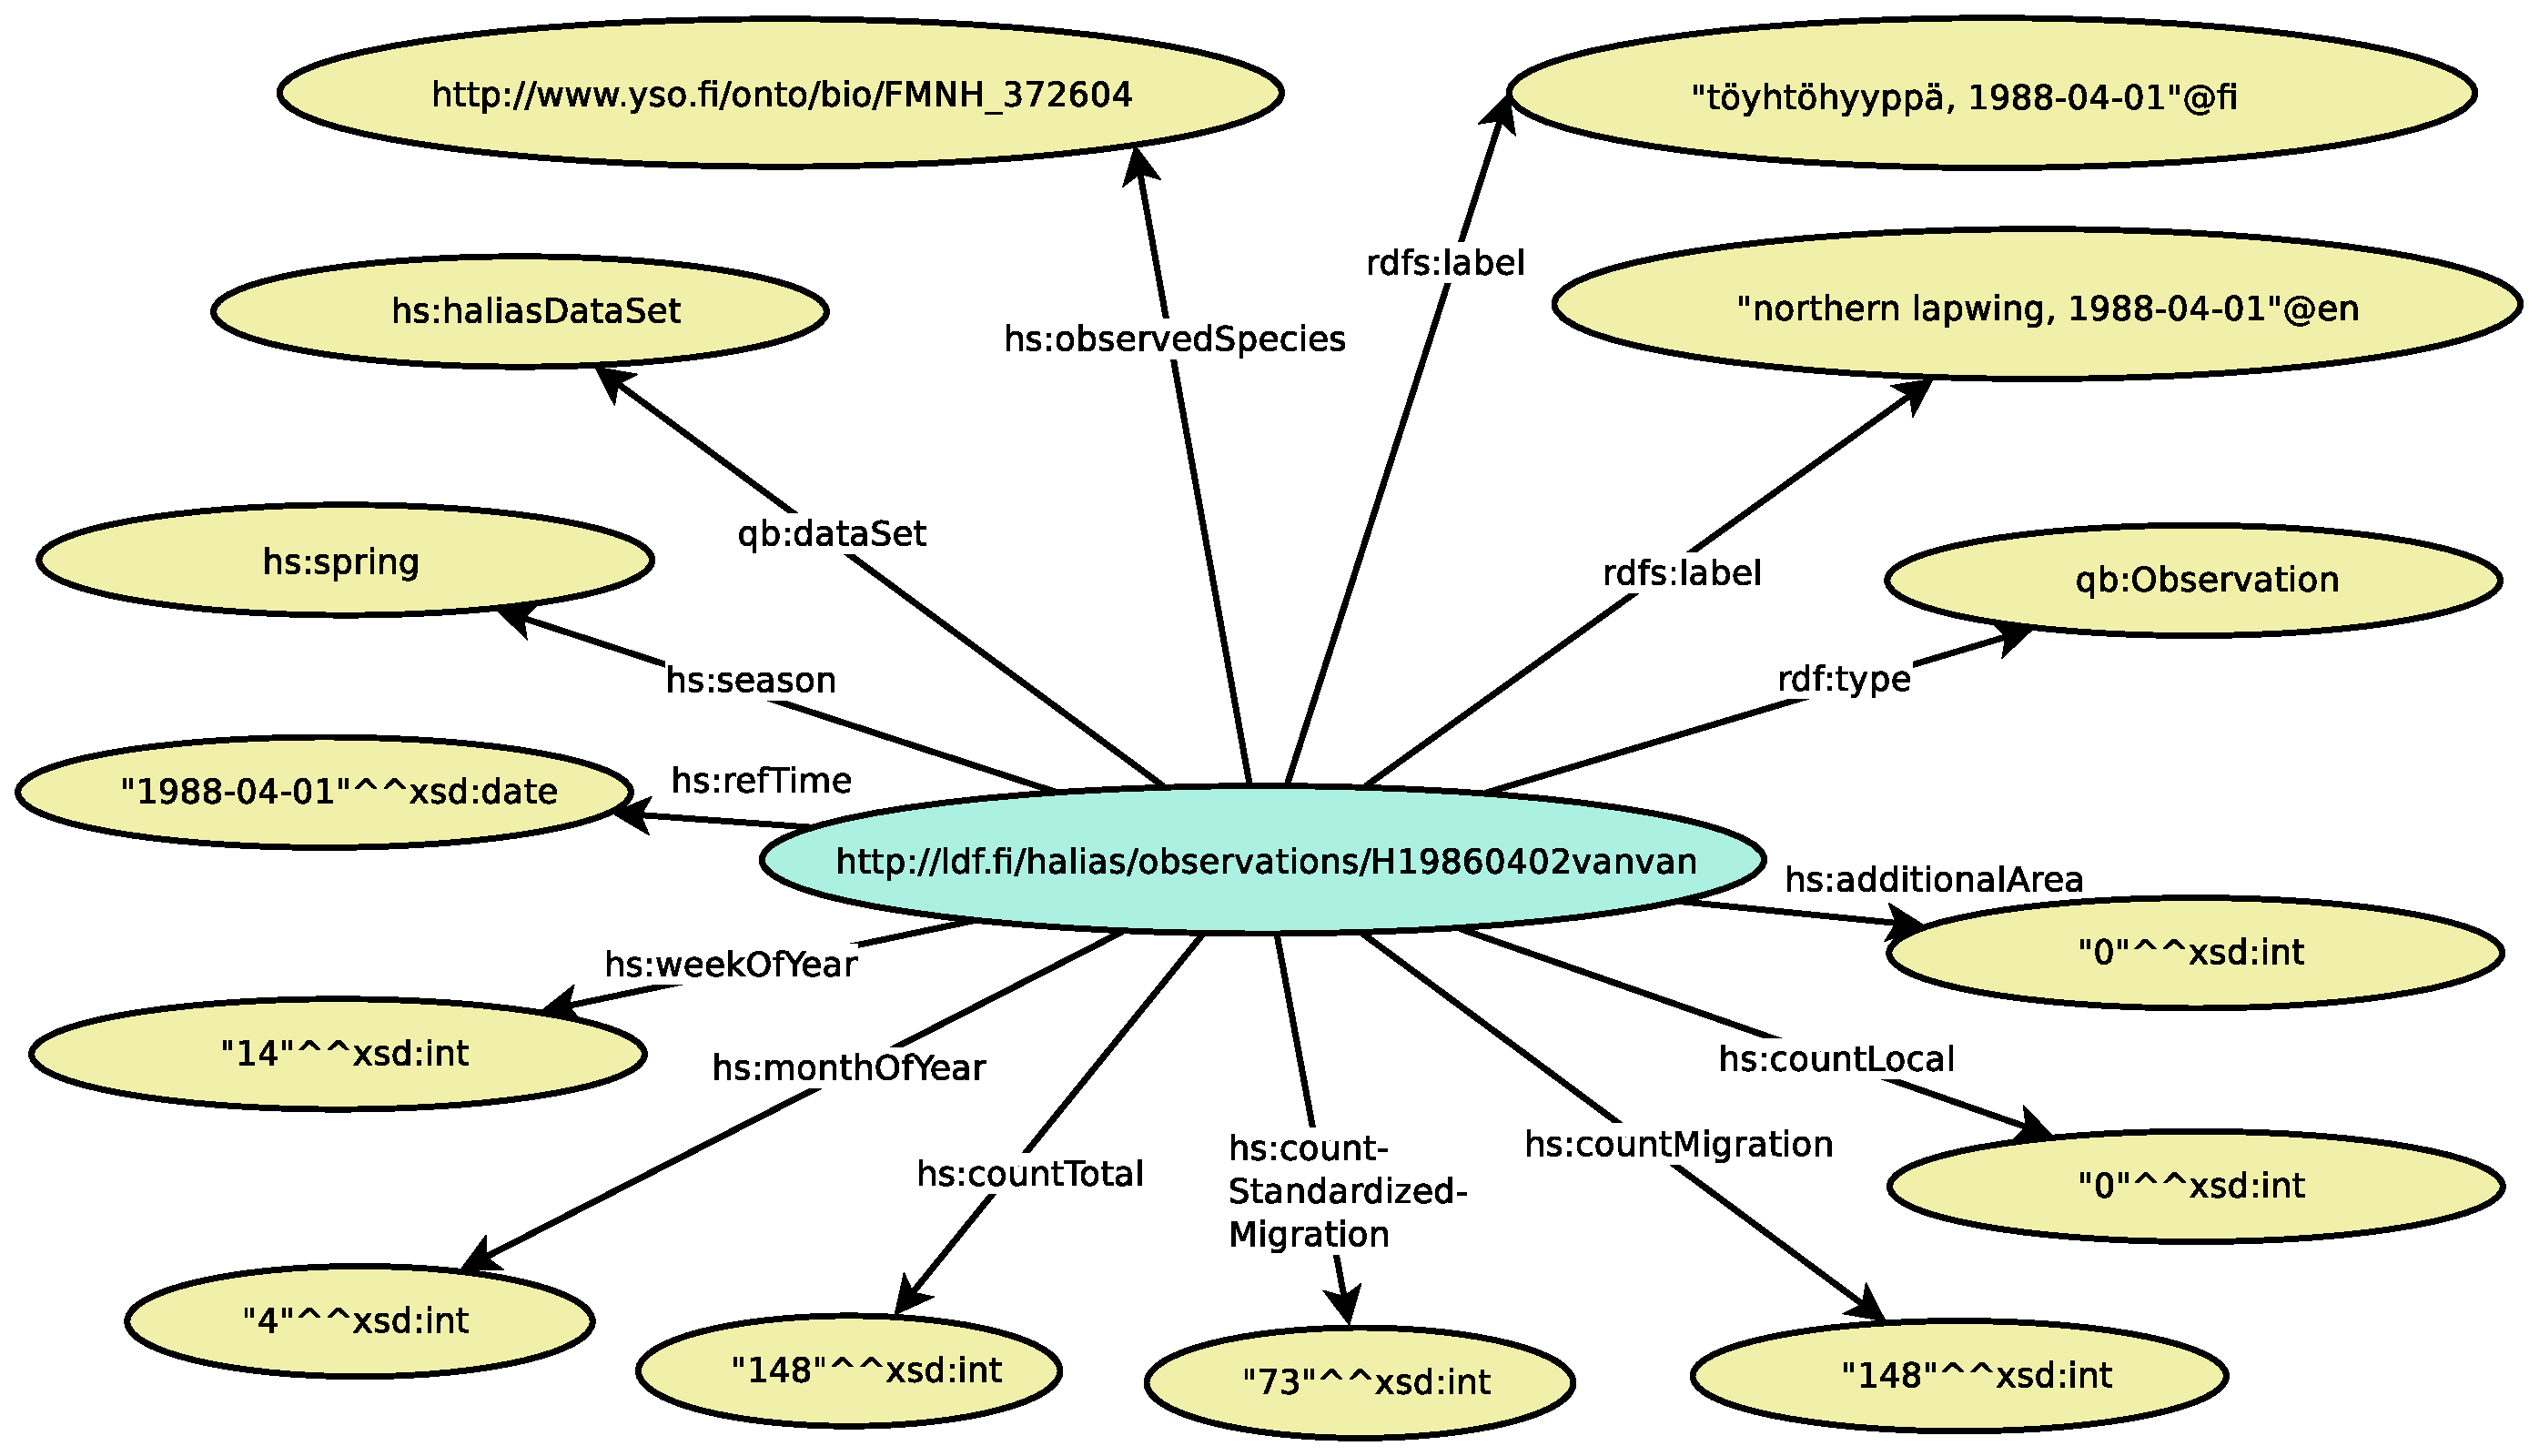
\includegraphics[clip=true, width=\textwidth]{havaintograafi}
\caption{Daily observation data of one species from one day in RDF format~\cite{koho2015gradu}.}
\label{fig: havaintograafi}
\end{figure}


%%%%%%%%%%%%%%%%%%%
\section{Methodology}
%%%%%%%%%%%%%%%%%%%

For association analysis we take a subset of the dimensions of the data cubes and transform these to market basket transactions or sequence database~\cite{tan2006introduction}. In this transformation it is easy to combine bird observations, weather observations and information from the used ontologies. The transformed data is stored in \emph{JSON} or text files, which is then read in when doing analysis.

We first analysed only the bird observations without any related information. Simple visualizations provide some insight into the occurence of different species. Frequent pattern mining was used to find the most frequently observed species and species combinations, without using the daily counts.

A sequential pattern discovery~\cite{tan2006introduction} attempt was also made using daily observed species as sequential patterns, where each year was used as a distinct sequence. The data set as sequence data was too large to get any good results in feasible time, and as the initial results did not seem to provide any interesting information, this attempt was not pursued further.
%7419 days, 378 taxa

The analysis is done using Python 3 and various modules. Initial examining the data was done mostly with \emph{IPython notebook}\footnote{\url{http://ipython.org/notebook.html}} and \emph{pandas} (Python Data Analysis Library)\footnote{\url{http://pandas.pydata.org/}}. Conversion from RDF uses \emph{RDFLib}\footnote{\url{https://github.com/RDFLib/rdflib}}. 

Pattern mining implementations are self-made and available online\footnote{\url{https://github.com/razz0/DataMiningProject}}. They include algorithms for finding frequent itemsets, frequent sequential patterns and rule generation. The algorithms are based on the \emph{Apriori algorithm}~\cite{tan2006introduction}.

The implemented pattern mining algorithms are somewhat memory efficient, but are computationally slow. They only use a single CPU core for all calculations and they use standard Python data types, which are flexible, but computationally inefficient. An attempt was made to optimize an Apriori based algorithm for speed, by first profiling the algorithm at execution time and finding the bottleneck, which is the pruning step.

We tried to optimize the pruning by using multiple processes, running in different CPU cores, using Python module Joblib\footnote{\url{https://pythonhosted.org/joblib/}}, which provides an improved interface to Python standard library \emph{multiprocessing} module. However, the processes running in parallel cannot access shared resources in memory, leading to extensive copying of large data structures and longer execution times. This could be overcome by switching to use data structures from NumPy\footnote{\url{http://www.numpy.org/}}, which are optimized for speed and allow shared access for multiple processes.

\emph{Orange Data Mining Toolbox}\footnote{\url{http://orange.biolab.si/}} was also tried for analysis, but it wasn't able to cope with large market basket transaction datasets.



%%%%%%%%%%%%%%%%%%%
\section{Results}
%%%%%%%%%%%%%%%%%%%

In this section we look at results of applying data mining methods to the dataset.



\subsection{Visualization}
%%%%%%%%%%%%%%%%%%%

\begin{figure}[htb]
\centering
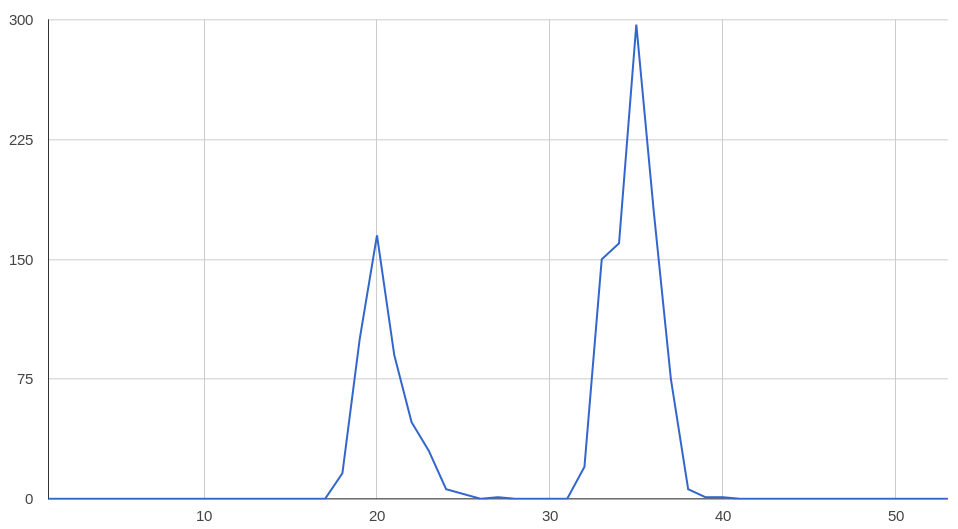
\includegraphics[clip=true, width=0.9\textwidth]{embhor_weeks}
\caption{Yearly occurence of ortolan bunting. X-axis contains week number, y-axis contains total observed individuals for week number.}
\label{fig: embhor_weeks}
\end{figure}

Visualizations of the data can easily convey important patterns in the data. Yearly occurence of species <peltosirkku, \emph{Emberiza hortulana}, ortolan bunting> if given in figure \ref{fig: embhor_weeks}. This shows a common yearly occurence of a migratory species not found at the bird observatory during breeding season. Most species are more frequent during autumn migration than during spring migration~\cite{lehikoinen2000phenology}.

%\begin{figure}[htb]
%\centering
%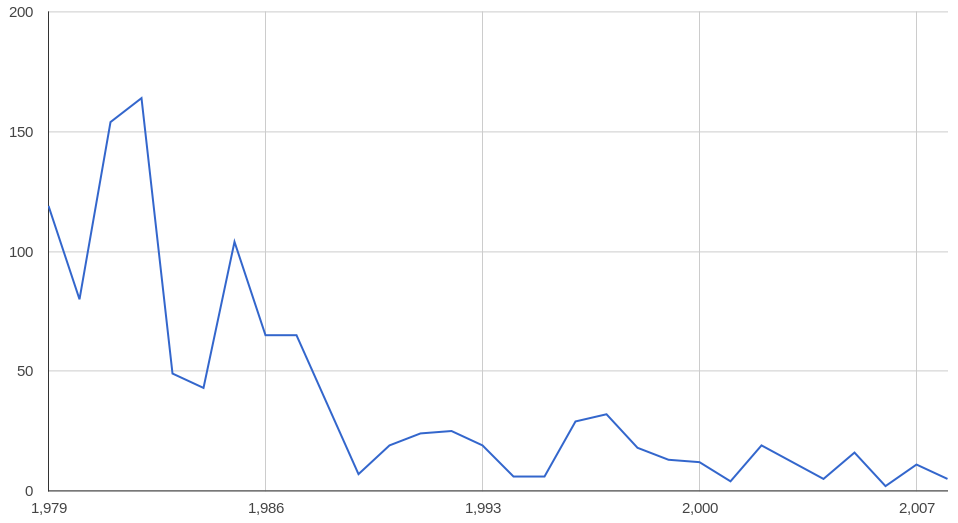
\includegraphics[clip=true, width=\textwidth]{embhor_years}
%\caption{embhor years}
%\label{fig: embhor_years}
%\end{figure}

%\begin{figure}[htb]
%\centering
%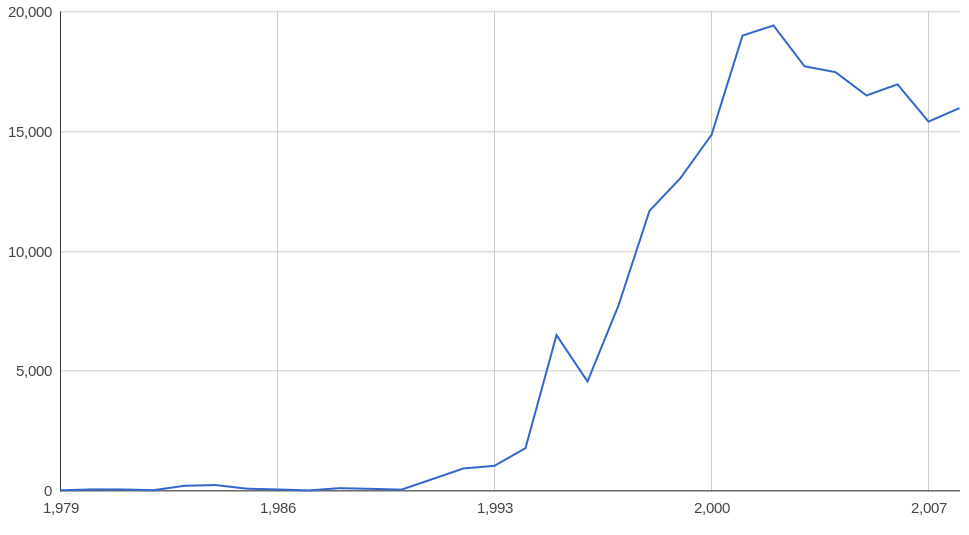
\includegraphics[clip=true, width=\textwidth]{phacar_years}
%\caption{phacar years}
%\label{fig: phacar_years}
%\end{figure}

%\begin{figure}[htb]
%\centering
%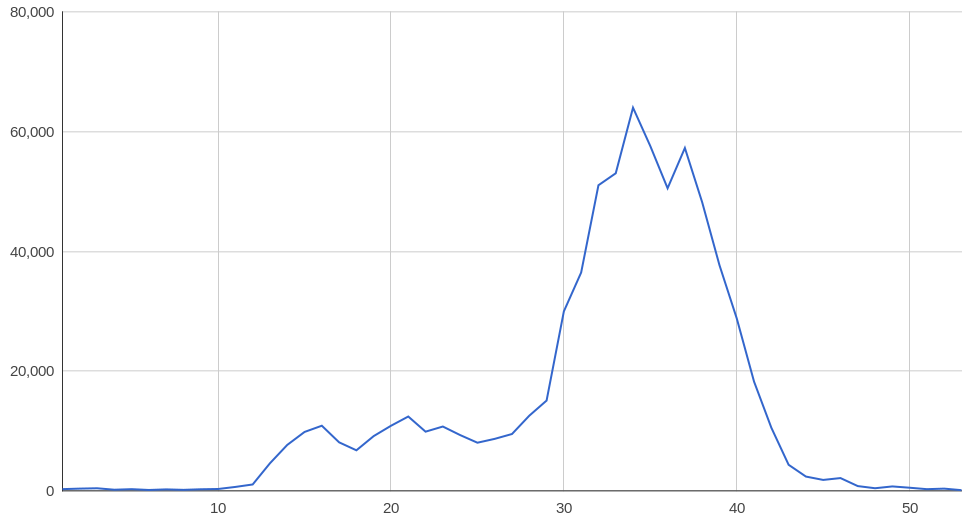
\includegraphics[clip=true, width=\textwidth]{phacar_weeks}
%\caption{phacar weeks}
%\label{fig: phacar_weeks}
%\end{figure}



\subsection{Frequent itemsets}
%%%%%%%%%%%%%%%%%%%

By using an algorithmic analysis of the dataset using daily observed species as market basket transactions, we can examine the most commonly observed species and species combinations. An implementation of Apriori algorithm was used to get itemsets that occur frequently in the transactions.

The most common species is <varis, \emph{Corvus corone}, carrion crow> with support 0.951. For support $0.5$, the largest frequent itemset consists of the following species:

%\begin{itemize}
\hangindent=0.7cm
<harmaalokki, \emph{Larus argentatus}, herring gull>, \\
<isokoskelo, \emph{Mergus merganser}, goosander/common merganser>, \\
<kalalokki, \emph{Larus canus}, mew gull>, \\
<merilokki, \emph{Larus marinus}, great black-backed gull>, \\
<sinisorsa, \emph{Anas platyrhynchos}, mallard>, \\
<sinitiainen, \emph{Parus caeruleus}, blue tit>, \\
<talitiainen, \emph{Parus major}, great tit>, \\
<telkkä, \emph{Bucephala clangula}, common goldeneye>, \\
<varis, \emph{Corvus corone}, carrion crow>, \\
<viherpeippo, \emph{Carduelis chloris}, european greenfinch> \\
%\nohang
%\end{itemize}

This is the largest combination of species that is observed in half of the observation days. These species are very common and observable almost all year round. Individually all of the listed species have support over $0.75$.



\subsection{Association rules}
%%%%%%%%%%%%%%%%%%%

We can create some association rules~\cite{tan2006introduction} that better explain the occurence of species at same dates. Examples of association rules with species <uuttukyyhky, \emph{Columba oenas}, stock dove> and <sepelkyyhky, \emph{Columba palumbus}, woodpigeon>, are shown in table \ref{fig: obs_itemset_rules}, which contains some rules with their measures~\cite{tan2006introduction} for confidence, support, lift and IS measure. The direction of the rule influences some of the given measures, but not all. Confidence is a frequentistic probability of the consequent happening if the antecedent has happened. So if a stock dove is observed it's very likely that a woodpigeon is also observed during the day, but not the other way around. Support gives the ratio of itemsets that contain both the antecedent and the consequent. Lift measures if the antecedent and consequent are dependent of each other, where value 1 implies independence. So woodpigeon and stock dove are strongly dependent according to the observations. The IS measure is large when lift and support are large.

\begin{table}[ht]
\centering
\begin{tabularx}{\textwidth}{| >{\hsize=2.4\hsize}X | >{\hsize=0.7\hsize}X | >{\hsize=0.7\hsize}X | >{\hsize=0.5\hsize}X | >{\hsize=0.7\hsize}X |}
  \hline
  \textbf{Rule} & \small \textbf{Con\-fi\-den\-ce} & \small \textbf{Sup\-port} & \small \textbf{Lift} & \small \textbf{IS measure}\\
  \hline
  \small
  \{woodpigeon\}
  $\rightarrow$
  \{stock dove\}
  & 0.49 & 0.22 & 1.86 & 0.63 \\
  \hline
  \small
  \{stock dove\}
  $\rightarrow$
  \{woodpigeon\}
  & 0.82 & 0.22 & 1.86 & 0.63 \\
  \hline
\end{tabularx}
\caption{Some association rules of species occurence at same dates.}
\label{fig: obs_itemset_rules}
\end{table}



\subsection{Analysing species itemsets}
%%%%%%%%%%%%%%%%%%%

For another type of analysis we created itemsets of all observed species. This creates 302 itemsets which consist of species name, its' characteristics, conservation status and commonness measure at Halias. All of the information are represented as strings. Many species lack characteristics annotations and for those species the itemsets are rather small.

All used species information is present in the taxon ontology and we transform the information into the itemsets as strings. Analysing these itemsets as market basket transactions we can infer frequent rules, but these mostly tell us about the used characteristics ontology and its' annotations.

Table \ref{fig: species_itemsets} shows two examples of a frequent generated rule with the rules' descriptive measures.
The ''Late spring -- early summer'' and ''Late summer -- autumn'' are part of the characteristics ontology, describing seasonal occurence of the species in Finland.

\begin{table}[htb]
\centering
\begin{tabularx}{\textwidth}{| >{\hsize=3.2\hsize}X | >{\hsize=0.5\hsize}X | >{\hsize=0.4\hsize}X | >{\hsize=0.3\hsize}X | >{\hsize=0.6\hsize}X |}
  \hline
  \textbf{Rule} & \small \textbf{Con\-fi\-den\-ce} & \small \textbf{Sup\-port} & \small \textbf{Lift} & \small \textbf{IS measure}\\
  \hline
  \small
  \{Late spring -- early summer, beak dark, head multicoloured, iris dark, upperside atleast 2-coloured\}
  $\rightarrow$
  \{Late summer -- autumn\} 
  & 0.99 & 0.51 & 1.26 & 0.80 \\
  \hline
  \small
  \{Common species at Halias\}
  $\rightarrow$
  \{Late spring -- early summer, Late summer -- autumn\} 
  & 0.93 & 0.51 & 1.19 & 0.78 \\
  \hline
\end{tabularx}
\caption{Two examples of frequent association rules generated from species itemsets.}
\label{fig: species_itemsets}
\end{table}



\subsection{Including weather variables}
%%%%%%%%%%%%%%%%%%%%%%%%%%%%%%%%%%%%%%%%%%%%%%%%%%%%

The species itemsets were further processed by leaving out all taxa that don't have characteristics annotations, and enriching the itemsets with the names of upper levels of taxon hierarchy. After this process we have a total of 239 itemsets, which are all created of species, as other taxonomic ranks lack characteristics annotations.

For each species we also add an average of the weather variables measured each day from sunrise to sunset and weight them with the total daily count of the species. So we get an average weather condition in which the species has been observed. All of the averaged weather variables were categorized in three categories: ''low'', ''average'' and ''high''. The categories contain respectively the lowest, middle and highest third of all numbers. The limits of the categories are shown in table \ref{fig: weather cats}.

\begin{table}[htb]
\centering
\begin{tabularx}{\textwidth}{| >{\hsize=1.0\hsize}X | >{\hsize=1.0\hsize}X | >{\hsize=1.0\hsize}X | >{\hsize=1.0\hsize}X |}
  \hline
  \textbf{Variable} & \textbf{Low} & \textbf{Average} & \textbf{High} \\
  \hline
  \textbf{Pressure} & [994.3, 1013.0] & (1013.0, 1014.5] & (1014.5, 1039.0] \\
  \textbf{Cloud cover} & [0.0, 3.9] & (3.9, 4.5] & 4.5, 8.0] \\ 
  \textbf{Humidity} & [56.0, 79.7] & (79.7, 81.8]        & (81.8, 93.7] \\
  \textbf{Rainfall} & [0.0, 1.0] & (1.0, 1.4]          & (1.4, 18.0] \\ 
  \textbf{Temperature} & [-2.4, 8.4]     & (8.4, 12.1]         & (12.1, 20.0] \\ 
  \textbf{Wind speed} & [0.1, 8.0]      & (8.0, 18.8]         & (18.8, 2109.0] \\
  \hline
\end{tabularx}
\caption{Weather variable category limits derived from averaged weather variables by dividing them into three equally sized chunks.}
\label{fig: weather cats}
\end{table}

The itemset sizes vary between each species, consisting of 36 to 66 items. The size depends on the amount of characteristics annotations, how many upper taxa it has in the taxon ontology and whether it has a conservation status or not.

We generated association rules from these species itemsets using an Apriori-based algorithm. The rule generation included using frequent itemsets with minimum support $0.3$ and using minimum confidence of $0.5$, which resulted in $105,949$ association rules. Some examples of the generated rules with their measurements are given in table \ref{fig: species_itemsets_2_rules}. The last rule in the table is one that has very high lift, indicating a strong dependency between species of the order <varpuslinnut, \emph{Passeriformes}, passerine> and some characteristics.

\begin{table}[htb]
\centering
\begin{tabularx}{\textwidth}{| >{\hsize=3.2\hsize}X | >{\hsize=0.5\hsize}X | >{\hsize=0.4\hsize}X | >{\hsize=0.3\hsize}X | >{\hsize=0.6\hsize}X |}
  \hline
  \textbf{Rule} & \small \textbf{Con\-fi\-den\-ce} & \small \textbf{Sup\-port} & \small \textbf{Lift} & \small \textbf{IS measure}\\
  \hline
  \small
  \{Rare at Halias\}
  $\rightarrow$
  \{Head multicoloured, late summer -- autumn, upperside atleast two-coloured, late spring -- early summer\} 
  & 0.89 & 0.30 & 0.99 & 0.55 \\
  \hline
  \small
  \{Common at Halias, walks\}
  $\rightarrow$
  \{Wind speed average, underside atleast two-coloured\} 
  & 0.80 & 0.38 & 1.02 & 0.62 \\
  \hline
  \small
  \{Beak dark, iris dark\}
  $\rightarrow$
  \{Upperside atleast two-coloured, common at Halias, underside atleast two-coloured\} 
  & 0.63 & 0.45 & 1.09 & 0.70 \\
  \hline
  \small
  \{Passerine\}
  $\rightarrow$
  \{Head multicoloured, legs short, late summer -- autumn, beak sharp, iris dark, upperside atleast two-coloured, late spring -- early summer\} 
  & 0.84 & 0.31 & 2.09 & 0.81 \\
  \hline
\end{tabularx}
\caption{Some association rules generated from species itemsets.}
\label{fig: species_itemsets_2_rules}
\end{table}

% TODO: Sääntöjen vertailu: 
% valtava -> matala ilmanpaine
% valtava -> korkea ilmanpaine

% valtava -> tuulen nopeudet

Table \ref{fig: handmade rules} shows some relationships between bird sizes and weather variables. From the confidence and lift we can see that the they correlate to air pressure with different sign depending on the bird size. Larger birds are more dependent on clear weather when migrating, and higher air pressure indicates clearer weather. Small birds are not very much dependent on the weather when migrating, and also local rainfall, which is associated with low air pressure, may cause migrants to pause the migration, at which time they may be feeding locally at Halias and thus be easily observed. The rules seem to support these assumptions.
Also all bird of prey of different sizes migrate mostly during clear, sunny weather and this can be stronly seen in association rules including the order <petolinnut, \emph{Falconiformes}, birds of prey>. No species of the order has an average observation air pressure in the ''low'' category, although some species of the order are not included in the analysis as they are lacking characteristics annotations and thus are not included in the itemsets.


\begin{table}[htb]
\centering
\begin{tabularx}{\textwidth}{| >{\hsize=3.2\hsize}X | >{\hsize=0.5\hsize}X | >{\hsize=0.4\hsize}X | >{\hsize=0.3\hsize}X | >{\hsize=0.6\hsize}X |}
  \hline
  \textbf{Rule} & \small \textbf{Con\-fi\-den\-ce} & \small \textbf{Sup\-port} & \small \textbf{Lift} & \small \textbf{IS measure}\\
  \hline
  \small
  \{Size huge\} $\rightarrow$ \{Air pressure low\} 		& 0.15 & 0.01 & 0.45 & 0.06 \\
  \hline
  \small
  \{Size huge\} $\rightarrow$ \{Air pressure average\} 	& 0.38 & 0.02 & 1.16 & 0.16 \\
  \hline
  \small
  \{Size huge\} $\rightarrow$ \{Air pressure high\} 	& 0.46 & 0.03 & 1.40 & 0.19 \\
  \hline
  \small
  \{Size small\} $\rightarrow$ \{Air pressure low\} 	& 0.38 & 0.13 & 1.11 & 0.39 \\
  \hline
  \small
  \{Size small\} $\rightarrow$ \{Air pressure average\} & 0.40 & 0.14 & 1.21 & 0.41 \\
  \hline
  \small
  \{Size small\} $\rightarrow$ \{Air pressure high\} 	& 0.22 & 0.08 & 0.67 & 0.23 \\
  \hline
  \small
  \{Bird of prey\} $\rightarrow$ \{Air pressure low\} 	& 0.0 & 0.0 & 0.0 & 0.0 \\
  \hline
  \small
  \{Bird of prey\} $\rightarrow$ \{Air pressure average\} 	& 0.39 & 0.03 & 1.18 & 0.19 \\
  \hline
  \small
  \{Bird of prey\} $\rightarrow$ \{Air pressure high\} 	& 0.61 & 0.05 & 1.85 & 0.29 \\
  \hline
\end{tabularx}
\caption{Some association rules between bird sizes and weather variables.}
\label{fig: handmade rules}
\end{table}


%%%%%%%%%%%%%%%%%%%
\section{Conclusions}
%%%%%%%%%%%%%%%%%%%

Data mining approach can be applied to biodiversity data to find interesting patterns. There are numerous possibilities how to organize the data into itemsets for pattern mining. By grouping relevant information of each species to a single itemset, we can efficiently analyse them for frequent patterns. Semantically linked datasets and related ontologies can be used to easily build the itemsets.

%%%%%%%%%%%%%%%%%%%
\section{Discussion}
%%%%%%%%%%%%%%%%%%%

It could be interesting for frequent rule generation to provide also monthly occurence at the bird observatory to species itemsets. The occurence information could use some quantitative categorization. This would allow for analysing which species characteristics are frequent during different months.

Also other kind of information, like a trend of yearly observation counts could be added to itemsets, to analyse what kind of trends do endangered species have. Also there could possibly be found unexpected association rules for species with clear negative or positive trends.

Directly including quantitative occurence data of each taxon in the daily observation itemsets could provide some interesting patterns.

\pagebreak

% --- References ---
%
% bibtex is used to generate the bibliography. The babplain style
% will generate numeric references (e.g. [1]) appropriate for theoretical
% computer science. If you need alphanumeric references (e.g [Tur90]), use
%
% \bibliographystyle{babalpha-lf}
%
% instead.

\bibliographystyle{babalpha-lf}
\bibliography{references-en}

\lastpage

\end{document}
